\documentclass[crop,tikz]{standalone}

\usepackage{amsmath}

% #1 = position, #2 = label
\newcommand{\drawnum}[2]{%
  \draw ({90-30*#1}:\radius) -- ({90-30*#1}:{\radius-\markersize});%
  \node at ({90-30*#1}:{(\radius-\markersize)*0.85}) {#2};%
}

\begin{document}
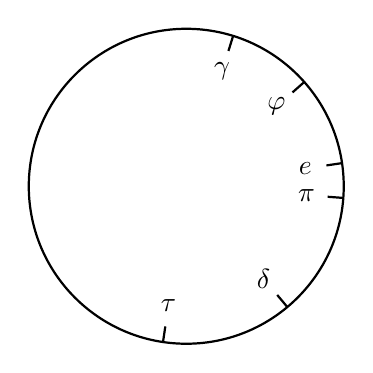
\begin{tikzpicture}[thick]
  \pgfmathsetmacro{\radius}{2}
  \pgfmathsetmacro{\markersize}{0.1*\radius}
  %
  \draw (0,0) circle (\radius);
  \drawnum{0.5772156649}{$\gamma$}        % Euler-Mascheroni constant
  \drawnum{1.61803}{$\varphi$}            % golden ratio
  \drawnum{2.71828}{$e$}                  % Euler's number
  \drawnum{3.14159}{$\pi$}                % pi
  \drawnum{6.28319}{$\tau$}               % tau = 2pi
  \drawnum{4.66920}{$\delta$}             % Feigenbaum constant
\end{tikzpicture}
\end{document}
